\section{Durchführung}
\label{sec:Durchführung}
\subsection{Aufbau}

In \autoref{fig:aufbau} ist der schematische Aufbau der genutzten Messapparatur dargestellt. 
\begin{figure}[H]
\centering
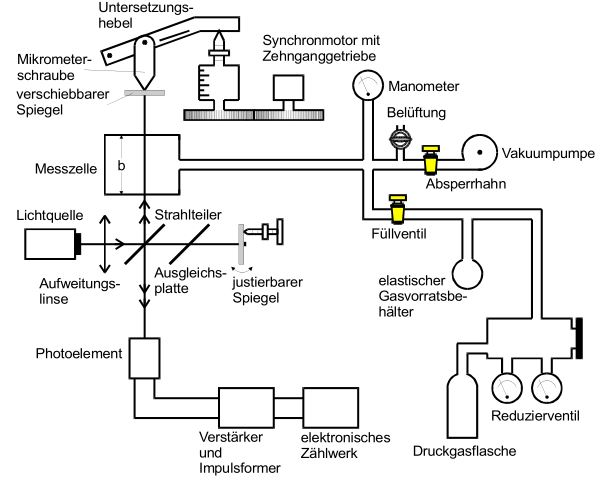
\includegraphics[width=\textwidth]{graphics/aufbau.JPG}
\caption{Schematischer Aufbau der genutzten Messapparatur \cite{anleitung}}
\label{fig:aufbau}
\end{figure}
\noindent
Die Wellenlänge des genutzten Lasers beträgt $\SI{635}{\nano\meter}$ und die Hebelübersetzung beträgt $1:5,046$
\subsection{Messvorgang}
Vor der eigentlichen Messung wird die Messapparatur kalibriert. Dabei werden die Spiegel so ausgerichtet, dass die einzelnen zu sehenden Lichtstreifen übereinander liegen. Als Hilfe wird bei der Justierung ein weißes Blatt Papier vor den Detektor gehalten, sodass die Lichtstreifen deutlicher zu sehen sind.

8 messreihen aufgenommen, Motor abwechselnd vor und zurück laufen gelassen
bei Geschwindigkeit 1, jeweils 5 mm range abgelesen an der
mikrometerschraube

Gleiche messweise diesmal mit druckänderung verursacht durch vakuumpumpe.
16 Messwerte 8 mal aufgepumpt 8 mal rausgelassen dabei drauf achten dass
die Änderung nicht zu schnell ist damit die richtige pulszahl gemessen
wird.
Übersetzung Wellenlänge
